\chapter{全景漫游的交互实现}
上文中通过对全景漫游与人的生理心理特性相互关系进行分析,梳理了以信息架构和功能模型为主导的可视化设计思路,为实际开发全景漫游项目奠定了基础。结合上述理论支持与作者实习实践所得经验,本章就某公司全景漫游系统开发为可视化交互示范案例进行分析。本案例将从需求定义、功能架构、交互模型定义出发,以实例开发为主线,通过界面设计和程序逻辑部分详细说明全景漫游的可视化实现过程,将理论与实践结合,从而提升全景漫游整体的使用交互体验。

\section{需求定义}
本例中的研究对象是一个包含商城内容、视频内容和基本交互场景的基于 web 技术的全景漫游系统。原始需求列表如下:
\begin{itemize}
	\item 满足基本全景漫游功能。因 web 环境受限,以直接在浏览器内打开所支持的操作为限,暂不考虑开发多种操作形式功能。
	\item 带有商城功能,实现互动场景的付费/免费使用。
	\item 支持全景视频的播放,基本功能类似普通播放器。
	\item 带有基本的用户设置功能。
\end{itemize}

根据以上原始需求,从价值需求、功能需求、数据需求等三个角度出发进行需求分析。

\subsection{价值需求分析}
该全景漫游系统的主要用户群为使用计算机或手持移动设备进行网页浏览的青少年群体。其用户特征为对新事物充满好奇心,愿意为良好的用户体验付出金钱成本,但缺点是对事物的专注度低,易于分心。

以该群体作为主要用户对象进行价值评估,按功能和用户的对应需求结合匹配,其价值需求如表\ref{tab:value}。

\begin{table}[htbp]
\centering
\caption{目标群体价值分析}
\vskip 5pt
\begin{tabular}{llll}
\toprule
功能点 & 用户需求 & 价值 \\
\midrule
新鲜感 & 体验到与其他应用不同的内容 & 高 \\
操作性 & 可以方便地了解并获取到所需体验的内容 & 中 \\
可信度 & 能够理解场景传达的信息并作出肯定答复 & 中 \\
丰富性 & 内容类别丰富、有不同难易层次可供选择 & 中 \\
可搜索 & 可以通过文本信息检索需要的项目 & 低 \\
可回溯 & 查看历史回放、收藏夹功能 & 低 \\
社交性 & 体验后愿意与别人分享使用体验 & 高 \\
\bottomrule
\end{tabular}
\label{tab:value}
\end{table}

根据分析,目标群体所期望的是一种不带有过多使用负担、随到随用、用完可离开也可进行分享的交互体验\endnote{陈圆. 手机应用软件界面体验设计研究[D].哈尔滨工程大学,2013.}
。

\subsection{功能需求分析}
据上述价值需求分析可得该全景漫游系统的功能需求,系统内的各种分类或是查找功能等,目的都是通过数据整理来让用户更好地发现场景并与其进行交互,如图\ref{fig:interaction}。经过整理分析以及结合软件开发难度等因素,可得功能需求表\ref{tab:func}。

\begin{figure}[htp]
\centering
\fbox{
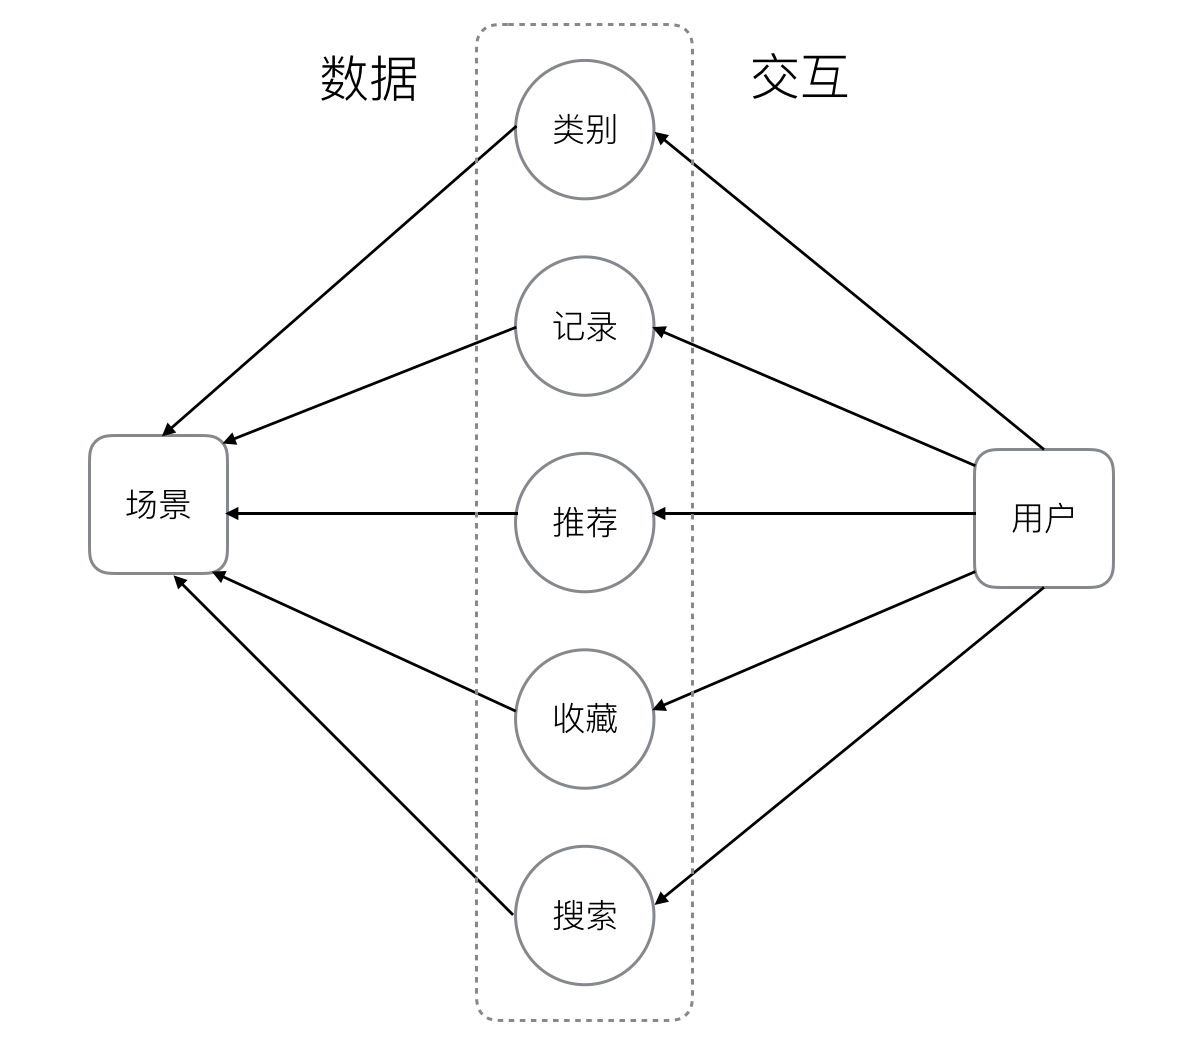
\includegraphics[width=.5\textwidth]{interaction}
}
\caption{用户通过多种形式发现场景}
\label{fig:interaction}
\end{figure}


\begin{table}[htp]
\centering
\caption{功能需求表}
\vskip 5pt
\begin{tabular}{lll}
\toprule
类别 & 功能点 & 描述 \\
\midrule
\multirow{3}{*}{主界面} & 推荐 & 进入推荐场景 \\
& 类别 & 按类别查看场景视频,可翻页,可进入类别界面 \\
& 应用 & 被固定的第三方开发的全景应用 \\
\midrule
\multirow{2}{*}{类别界面} & 列表 & 查看场景视频 \\
& 标签 & 切换类别 \\
\midrule
\multirow{2}{*}{应用界面} & 列表 & 展示第三方应用 \\
& 标签 & 切换类别 \\
\midrule
\multirow{2}{*}{设置界面} & 通用设置 & 提醒、关于 \\
& 个人偏好 & 账户设置、收藏夹、使用记录 \\
\midrule
\multirow{3}{*}{全局导航} & 返回 & 返回上一层 \\
& 主页 & 返回主界面 \\
& 搜索 & 唤起全局或当前类别搜索 \\
\midrule
\multirow{4}{*}{场景} & 定位 & 回到初始角度 \\
& 标签 & 标记为喜爱或讨厌、帮助改进推荐质量 \\
& 分享 & 分享页面至社交媒体 \\
& 解锁 & 解锁付费内容 \\
\bottomrule
\end{tabular}
\label{tab:func}
\end{table}

\subsection{数据需求分析}
根据上述功能需求可知,整个系统中最小的个体单位是场景,数据集合的建立是以场景为中心的。则该全景漫游系统的数据需求以单个场景的数据集出发,进行数据字段的定义,见表\ref{tab:data}。

\begin{table}[htp]
\centering
\caption{场景数据集}
\vskip 5pt
\begin{tabular}{lll}
\toprule
类别 & 字段 & 描述 \\
\midrule
\multirow{4}{*}{基础信息}& 名称 & 场景名称 \\
& 性质 & 视频、游戏、应用等 \\
& 标签 & 场景分类(如科幻、太空等) \\
& 介绍 & 场景简短介绍 \\
\midrule
\multirow{4}{*}{自然信息}& 容量 & 场景占用空间大小,以 kb 计 \\
& 创建日期 & 场景创建日期 \\
& 时长 & 仅对视频场景有效 \\
& 地理信息 & 场景录入地点 \\
\midrule
\multirow{3}{*}{人为信息}& 价格 & 免费、收费、部分收费 \\
& 分级 & 年龄限制、内容限制 \\
& 可用 & 可用或不可用 \\
\bottomrule
\end{tabular}
\label{tab:data}
\end{table}

而作为交互界面,场景是用来服务于使用其的用户的,故数据需求也包含用户信息数据的模型,见表\ref{tab:user}。

\begin{table}[htp]
\centering
\caption{用户数据集}
\vskip 5pt
\begin{tabular}{lll}
\toprule
类别 & 字段 & 描述 \\
\midrule
\multirow{3}{*}{基本信息} & 名称 & 账户名称 \\
& 密码 & 账户密码 \\
& 邮箱 & 账户邮箱 \\
\midrule
\multirow{3}{*}{被动收集信息} & 观看记录 & 场景、时间、时长 \\
& 付费记录 & 场景、应用、视频即其价格 \\
& 操作记录 & 使用场景的有效信息 \\
\midrule
\multirow{3}{*}{主动输入信息} & 标签 & 标记喜恶、收藏 \\
& 偏好设置 & 使用设备、情景模式等 \\
\bottomrule
\end{tabular}
\label{tab:user}
\end{table}

\section{功能架构}
据上述需求分析,该全景漫游系统等功能架构表现两种核心功能:“发现功能”和“场景漫游”。

\subsection{发现功能}
\begin{itemize}
	\item \emph{浏览功能}:使用者在包括主界面内的各种类别界面内浏览场景相关信息,发现自己所想要体验的场景。
	\item \emph{搜索功能}:使用者需要即时搜索得到自己想要的信息。
	\item \emph{记录功能}:使用者可以查看自己的浏览历史和收藏内容。
	\item \emph{付费功能}:使用者需要支付一定成本来查看某些场景或场景的局部。
	\item \emph{自定义功能}:使用者可以通过设置来自定义系统偏好。
\end{itemize}

\subsection{场景漫游功能}

\begin{itemize}
	\item \emph{漫游功能}:使用者可以通过转向、仰头低头、注视等方式漫游整个场景。
	\item \emph{互动功能}:使用者可以通过转向、仰头低头、注视等方式漫与场景内特定物件进行互动。
	\item \emph{视频功能}:使用者可以以全景的形式观看特殊全景视频。
	\item \emph{标记功能}:使用者将场景标记自己的评价、收藏或是分享给其他人。
\end{itemize}

\section{交互模型}
交互模型即是一系列交互方式、模式、行为的总称,它定义了交互过程中交互的主体对象和行为方式。交互模型并没有准确的定义,因为根据不同的产品而言,交互行为的目的并不相同。例如,对于网站管理员而言,编写并输入网站内容是使用网站的目的,而对于一般浏览者而言,浏览网页上提供的信息则是其在该网站上行为的目的,故从不同角色和视角看待交互模型都会是不同的。而构建交互模型的主要目的则是指导交互设计的进行,则构建一个能同时被用户接受并符合一般软件开发规律的交互模型是十分重要的。

交互模型需要符合用户心智模型并在后续可以方便进行扩充。在该全景漫游系统中,其基本交互模型如图\ref{fig:scene}。

\begin{figure}[htp]
\centering
\fbox{
  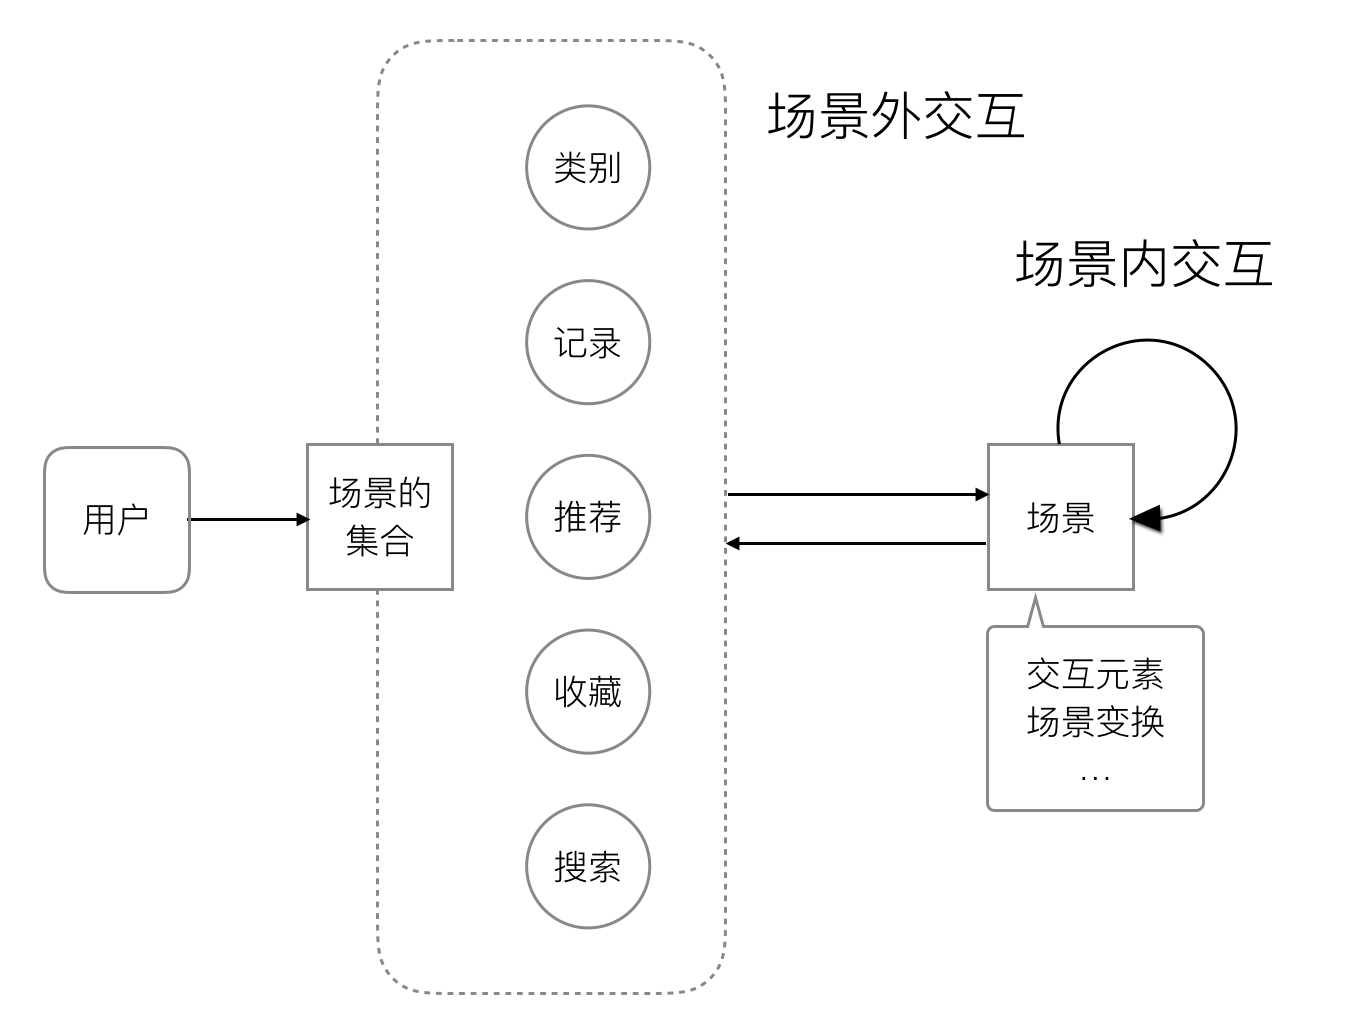
\includegraphics[width=.5\textwidth]{scene}
}
\caption{全景漫游系统的交互模型}
\label{fig:scene}
\end{figure}

\section{原型设计}
\subsection{类别界面设计}
上方为类别菜单,下边横长条为标签栏,可切换分类。底部为通用导航栏。如图\ref{fig:menu}。

\begin{figure}[htp]
\centering
\fbox{
  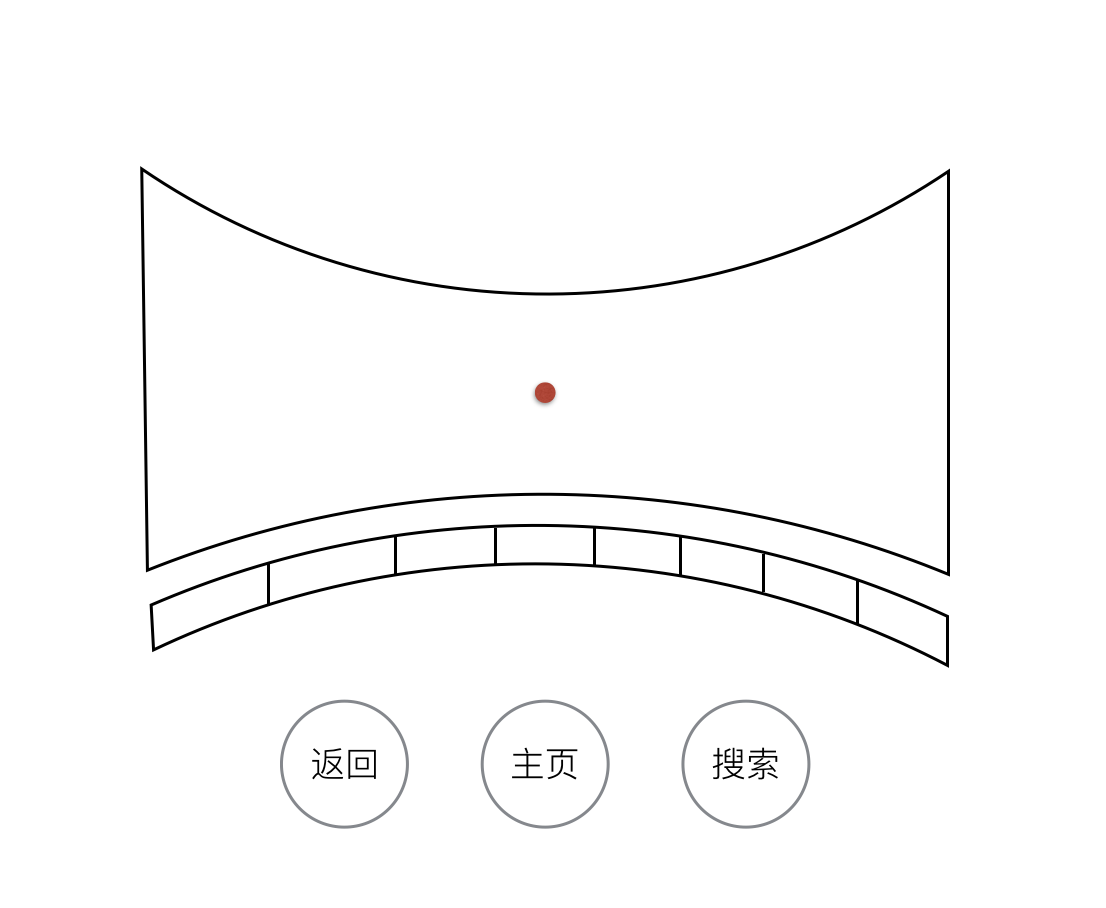
\includegraphics[width=.5\textwidth]{menu}
}
\caption{类别界面设计}
\label{fig:menu}
\end{figure}

\subsection{漫游界面设计}
\begin{itemize}
	\item 漫游界面带有紧急退出区域,只需注视 1~2 秒以上就可以紧急退出场景,避免眩晕加重。
	\item 可通过地面上的指示图标切换场景。
	\item 可通过场景中的热点区域查看详细信息。
\end{itemize}
如图\ref{fig:scenery}。

\begin{figure}[htp]
\centering
\fbox{
  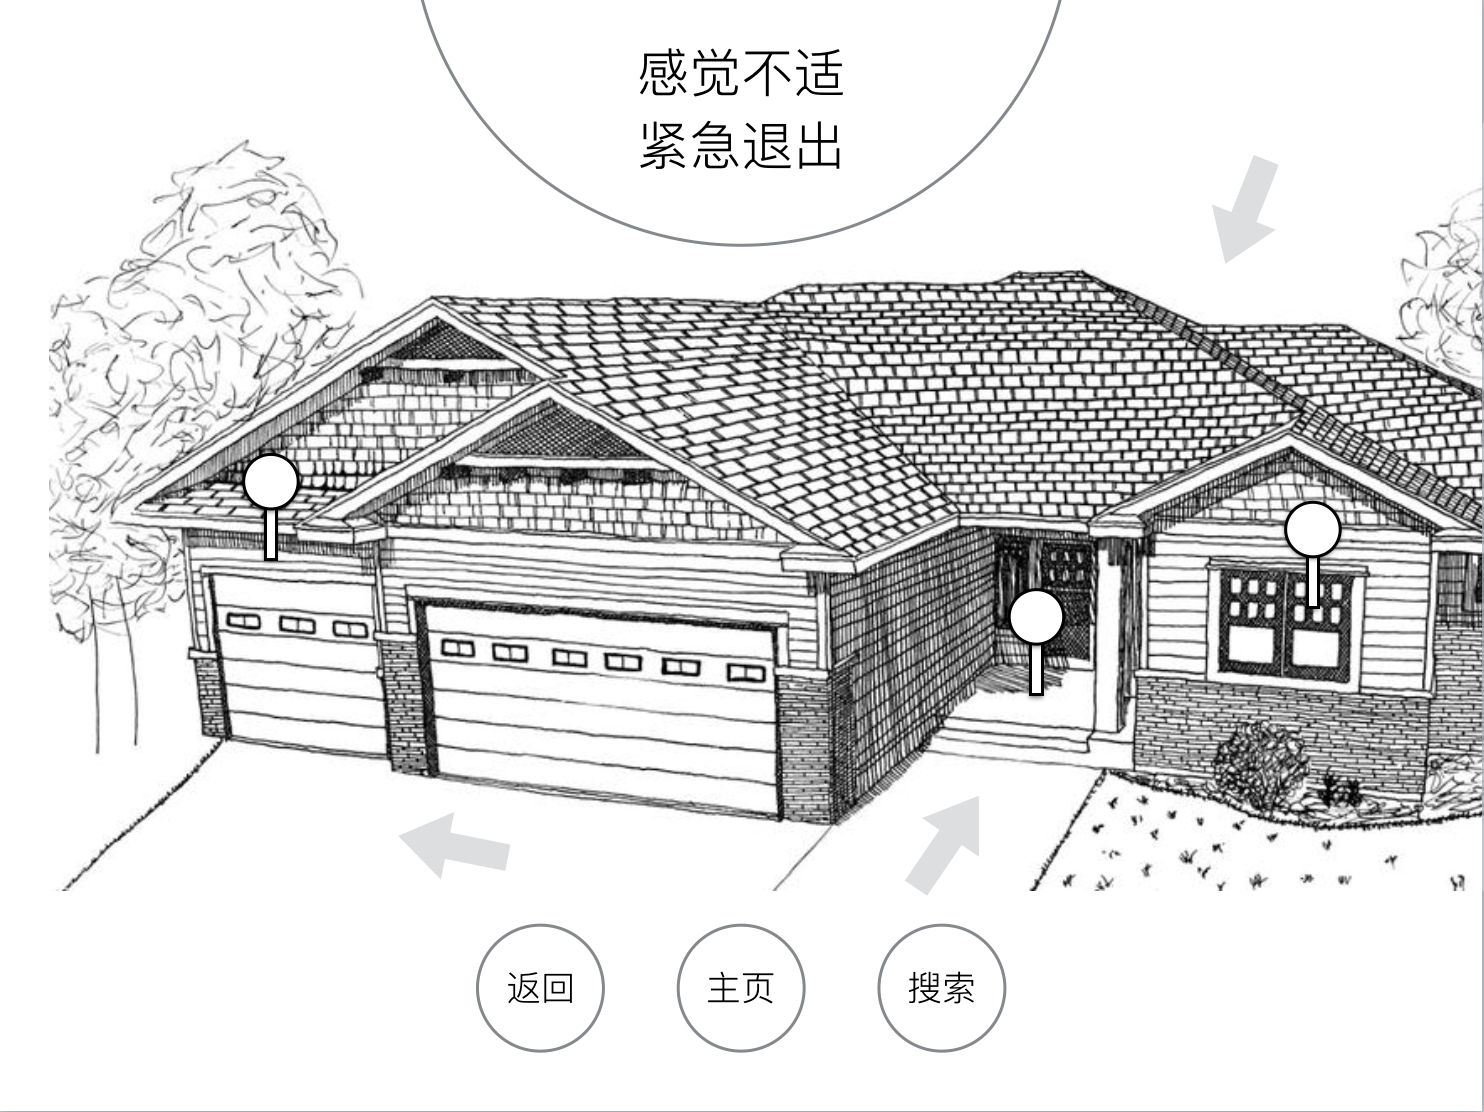
\includegraphics[width=.5\textwidth]{scenery}
}
\caption{漫游界面设计}
\label{fig:scenery}
\end{figure}

\subsection{设置界面设计}
设置界面可通过注视相关范围控件以调节参数,如图\ref{fig:setting}。

\begin{figure}[htp]
\centering
\fbox{
  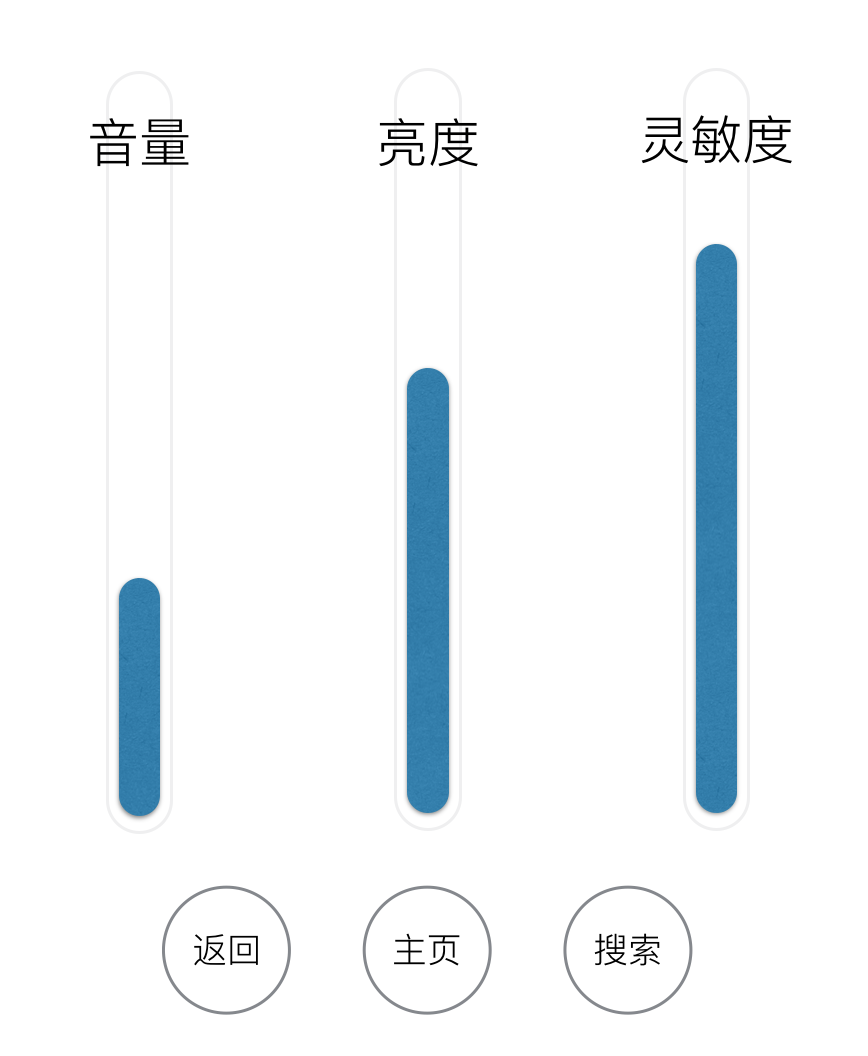
\includegraphics[width=.5\textwidth]{setting}
}
\caption{设置界面设计}
\label{fig:setting}
\end{figure}

\subsection{未完待续}

\section{程序示例}
本全景漫游系统采用 Mozilla 开源的 Aframe 框架进行开发,可满足普通计算机及移动设备通过浏览器进行使用。
\subsection{示例代码}
实现一个简单的可用鼠标或注视(Fuse)操作的小场景。


\emph{HTML}
\begin{lstlisting}[language=HTML]
<a-scene>
  <a-entity
    id="box" cursor="fuse:true;fuseTimeout:1000"
    geometry="primitive: box"
    material="color: blue">
    <a-box
      src="img/logo.jpg"
      position="0 3 -5"
      rotation="45 0 45"
      scale="2 2 2"
      id="box1">
      <a-animation
        attribute="position"
        begin="focus"
        to="0 2.2 -5"
        direction="normal"
        dur="2000">
      </a-animation>
    </a-box>
  </a-entity>

  <a-camera>
    <a-cursor></a-cursor>
  </a-camera>

  <a-plane 
    position="0 0 -4" 
    rotation="-90 0 0" 
    width="4" 
    height="4" 
    color="#7BC8A4">
  </a-plane>
  <a-sky color="#ECECEC"></a-sky>
</a-scene>
\end{lstlisting} 

\emph{JavaScript}
\begin{lstlisting}{language=JavaScript}
document.querySelector('#box').addEventListener('click', function(e){
  document.querySelector('#box1').emit('focus')
})
\end{lstlisting}
